\documentclass{beamer}

\usetheme{CambridgeUS}
\usecolortheme{dolphin}
\usefonttheme{serif}

\definecolor{rit@orange}{HTML}{F36E21}
\definecolor{rit@brown}{HTML}{513127}
\setbeamercolor{structure}{fg=rit@orange}
\setbeamercolor{palette primary}{fg=white, bg=rit@brown}
\setbeamercolor{palette secondary}{fg=rit@brown}
\setbeamercolor{palette tertiary}{fg=white, bg=rit@orange}
\setbeamercolor{titlelike}{fg=rit@brown}
\setbeamercolor{normal text}{fg=rit@brown}

\setbeamertemplate{enumerate}[circle]
\setbeamertemplate{items}[circle]

\AtBeginSection{\frame{\sectionpage}}

\setbeamertemplate{section page}
{
    \begin{centering}
    \begin{beamercolorbox}[sep=12pt,center]{part title}
    \usebeamerfont{section title}\insertsection\par
    \end{beamercolorbox}
    \end{centering}
}


\beamertemplatenavigationsymbolsempty

\logo{\includegraphics[width=0.50in]{img/astlogo}}

\pdfpageattr {/Group << /S /Transparency /I true /CS /DeviceRGB>>}

\usepackage{amsmath,amssymb,commath,physics}
\usepackage{float,subcaption}
\usepackage{xcolor}




\title[Variable Stars]{
  Fourier analysis of variable stars using regularized regression
}

\author[Daniel Wysocki]{
  Daniel Wysocki
}

\institute[RIT]{
  Rochester Institute of Technology
}


\date[Nov 23, 2015]{AST Graduate Seminar -- November 23rd, 2015}

\begin{document}

\maketitle


\begin{frame}{Light Curve}
  \begin{figure}[ht]
    \centering
    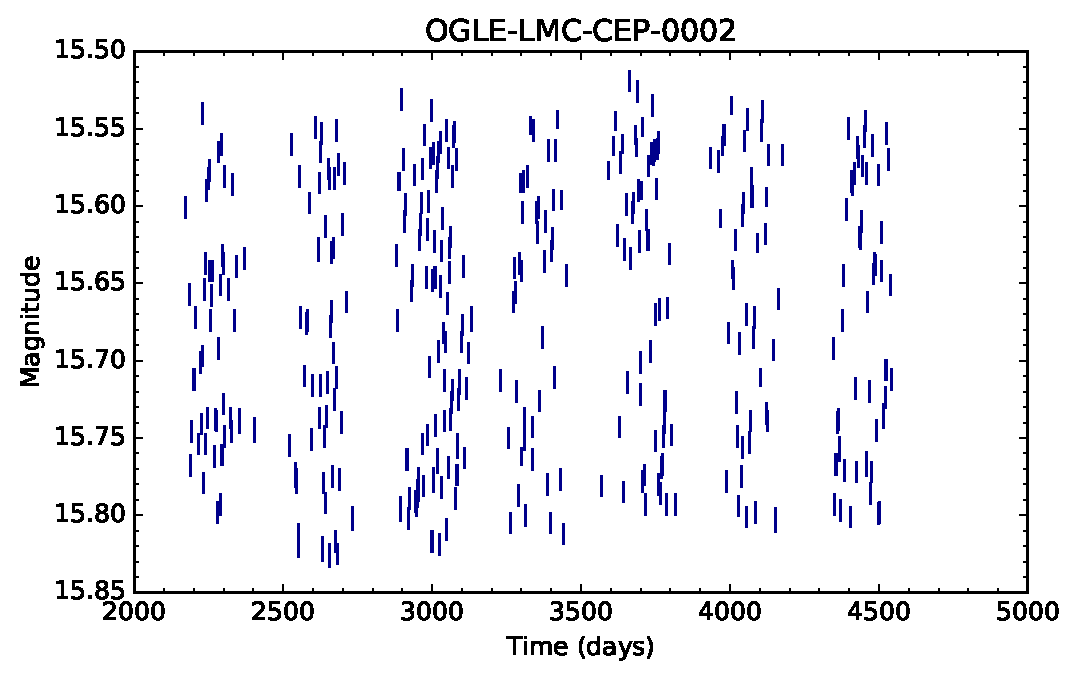
\includegraphics[width=0.8\textwidth]{img/lightcurve-raw}
    \caption{Raw light curve}
  \end{figure}
\end{frame}


\begin{frame}{Phased Light Curve}
  \begin{figure}[ht]
    \centering
    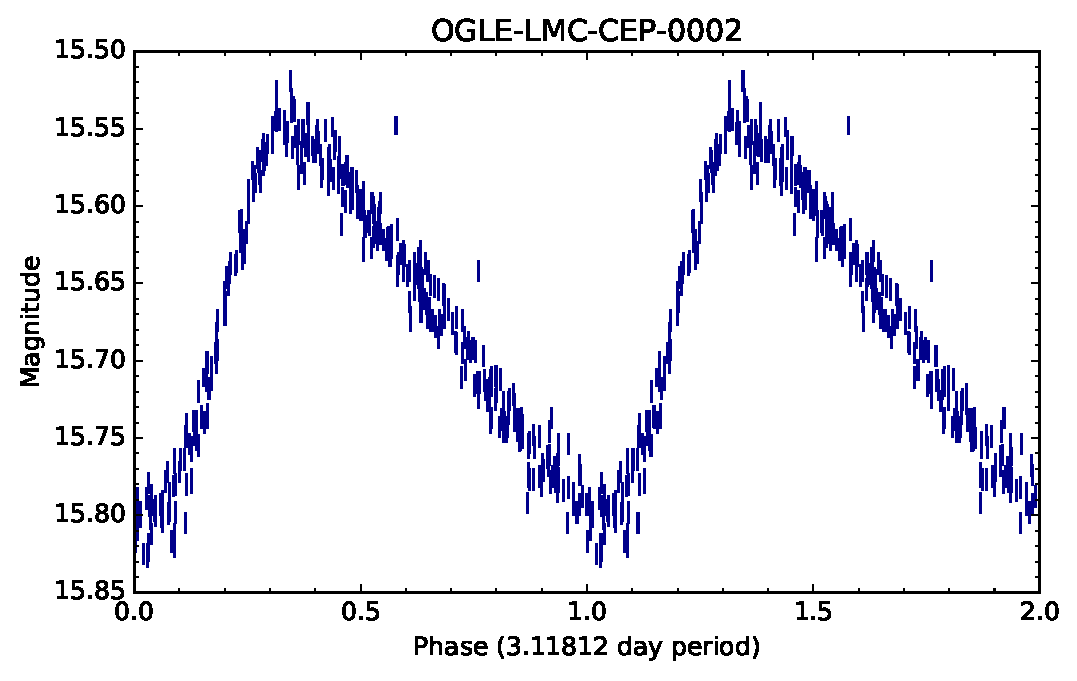
\includegraphics[width=0.8\textwidth]{img/lightcurve-phased}
    \caption{Phased light curve}
  \end{figure}
\end{frame}


\begin{frame}{Fourier Series}
  \begin{displaymath}
    m(t) = A_0 + \sum_{k=1}^n A_k \cos(k \omega t + \Phi_k)
  \end{displaymath}
\end{frame}


\begin{frame}{Unconstrained Regression Fit}
  \begin{figure}[ht]
    \centering
    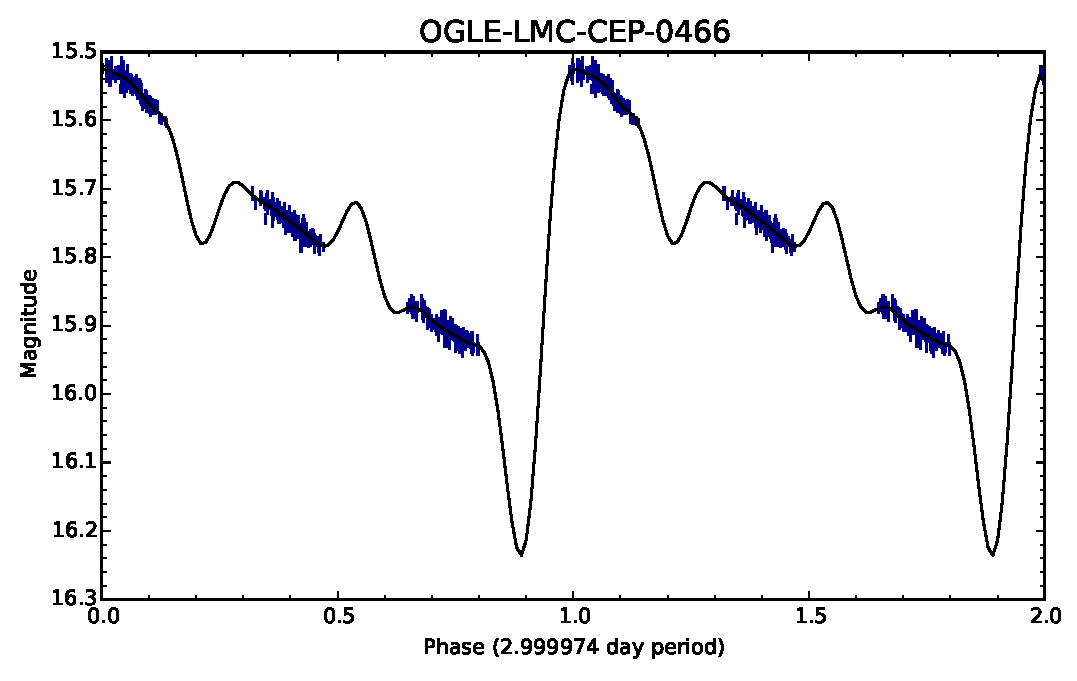
\includegraphics[width=0.8\textwidth]{img/lightcurve-ols}
    \caption{$10$th order fit using ordinary linear regression}
  \end{figure}
\end{frame}


\begin{frame}{Regularized Regression Fit}
  \begin{figure}[ht]
    \centering
    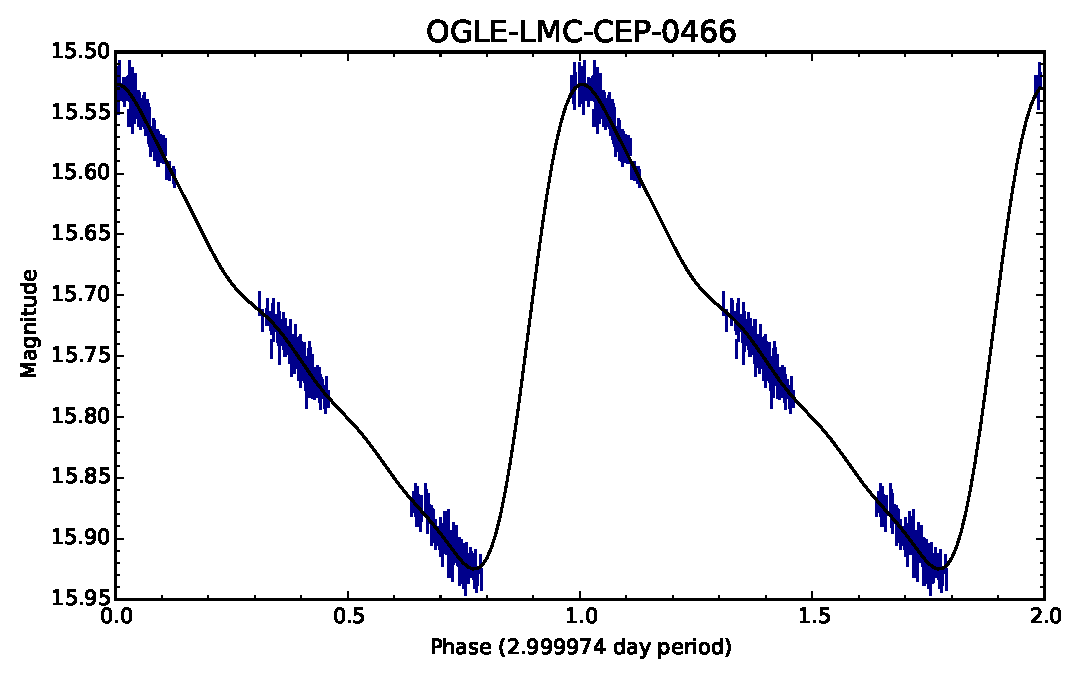
\includegraphics[width=0.8\textwidth]{img/lightcurve-lasso}
    \caption{$10$th order fit using LASSO and cross validation}
  \end{figure}
\end{frame}


\end{document}
